% Options for packages loaded elsewhere
\PassOptionsToPackage{unicode}{hyperref}
\PassOptionsToPackage{hyphens}{url}
%
\documentclass[
]{article}
\usepackage{amsmath,amssymb}
\usepackage{lmodern}
\usepackage{iftex}
\ifPDFTeX
  \usepackage[T1]{fontenc}
  \usepackage[utf8]{inputenc}
  \usepackage{textcomp} % provide euro and other symbols
\else % if luatex or xetex
  \usepackage{unicode-math}
  \defaultfontfeatures{Scale=MatchLowercase}
  \defaultfontfeatures[\rmfamily]{Ligatures=TeX,Scale=1}
\fi
% Use upquote if available, for straight quotes in verbatim environments
\IfFileExists{upquote.sty}{\usepackage{upquote}}{}
\IfFileExists{microtype.sty}{% use microtype if available
  \usepackage[]{microtype}
  \UseMicrotypeSet[protrusion]{basicmath} % disable protrusion for tt fonts
}{}
\makeatletter
\@ifundefined{KOMAClassName}{% if non-KOMA class
  \IfFileExists{parskip.sty}{%
    \usepackage{parskip}
  }{% else
    \setlength{\parindent}{0pt}
    \setlength{\parskip}{6pt plus 2pt minus 1pt}}
}{% if KOMA class
  \KOMAoptions{parskip=half}}
\makeatother
\usepackage{xcolor}
\usepackage[margin=1in]{geometry}
\usepackage{color}
\usepackage{fancyvrb}
\newcommand{\VerbBar}{|}
\newcommand{\VERB}{\Verb[commandchars=\\\{\}]}
\DefineVerbatimEnvironment{Highlighting}{Verbatim}{commandchars=\\\{\}}
% Add ',fontsize=\small' for more characters per line
\usepackage{framed}
\definecolor{shadecolor}{RGB}{248,248,248}
\newenvironment{Shaded}{\begin{snugshade}}{\end{snugshade}}
\newcommand{\AlertTok}[1]{\textcolor[rgb]{0.94,0.16,0.16}{#1}}
\newcommand{\AnnotationTok}[1]{\textcolor[rgb]{0.56,0.35,0.01}{\textbf{\textit{#1}}}}
\newcommand{\AttributeTok}[1]{\textcolor[rgb]{0.77,0.63,0.00}{#1}}
\newcommand{\BaseNTok}[1]{\textcolor[rgb]{0.00,0.00,0.81}{#1}}
\newcommand{\BuiltInTok}[1]{#1}
\newcommand{\CharTok}[1]{\textcolor[rgb]{0.31,0.60,0.02}{#1}}
\newcommand{\CommentTok}[1]{\textcolor[rgb]{0.56,0.35,0.01}{\textit{#1}}}
\newcommand{\CommentVarTok}[1]{\textcolor[rgb]{0.56,0.35,0.01}{\textbf{\textit{#1}}}}
\newcommand{\ConstantTok}[1]{\textcolor[rgb]{0.00,0.00,0.00}{#1}}
\newcommand{\ControlFlowTok}[1]{\textcolor[rgb]{0.13,0.29,0.53}{\textbf{#1}}}
\newcommand{\DataTypeTok}[1]{\textcolor[rgb]{0.13,0.29,0.53}{#1}}
\newcommand{\DecValTok}[1]{\textcolor[rgb]{0.00,0.00,0.81}{#1}}
\newcommand{\DocumentationTok}[1]{\textcolor[rgb]{0.56,0.35,0.01}{\textbf{\textit{#1}}}}
\newcommand{\ErrorTok}[1]{\textcolor[rgb]{0.64,0.00,0.00}{\textbf{#1}}}
\newcommand{\ExtensionTok}[1]{#1}
\newcommand{\FloatTok}[1]{\textcolor[rgb]{0.00,0.00,0.81}{#1}}
\newcommand{\FunctionTok}[1]{\textcolor[rgb]{0.00,0.00,0.00}{#1}}
\newcommand{\ImportTok}[1]{#1}
\newcommand{\InformationTok}[1]{\textcolor[rgb]{0.56,0.35,0.01}{\textbf{\textit{#1}}}}
\newcommand{\KeywordTok}[1]{\textcolor[rgb]{0.13,0.29,0.53}{\textbf{#1}}}
\newcommand{\NormalTok}[1]{#1}
\newcommand{\OperatorTok}[1]{\textcolor[rgb]{0.81,0.36,0.00}{\textbf{#1}}}
\newcommand{\OtherTok}[1]{\textcolor[rgb]{0.56,0.35,0.01}{#1}}
\newcommand{\PreprocessorTok}[1]{\textcolor[rgb]{0.56,0.35,0.01}{\textit{#1}}}
\newcommand{\RegionMarkerTok}[1]{#1}
\newcommand{\SpecialCharTok}[1]{\textcolor[rgb]{0.00,0.00,0.00}{#1}}
\newcommand{\SpecialStringTok}[1]{\textcolor[rgb]{0.31,0.60,0.02}{#1}}
\newcommand{\StringTok}[1]{\textcolor[rgb]{0.31,0.60,0.02}{#1}}
\newcommand{\VariableTok}[1]{\textcolor[rgb]{0.00,0.00,0.00}{#1}}
\newcommand{\VerbatimStringTok}[1]{\textcolor[rgb]{0.31,0.60,0.02}{#1}}
\newcommand{\WarningTok}[1]{\textcolor[rgb]{0.56,0.35,0.01}{\textbf{\textit{#1}}}}
\usepackage{graphicx}
\makeatletter
\def\maxwidth{\ifdim\Gin@nat@width>\linewidth\linewidth\else\Gin@nat@width\fi}
\def\maxheight{\ifdim\Gin@nat@height>\textheight\textheight\else\Gin@nat@height\fi}
\makeatother
% Scale images if necessary, so that they will not overflow the page
% margins by default, and it is still possible to overwrite the defaults
% using explicit options in \includegraphics[width, height, ...]{}
\setkeys{Gin}{width=\maxwidth,height=\maxheight,keepaspectratio}
% Set default figure placement to htbp
\makeatletter
\def\fps@figure{htbp}
\makeatother
\setlength{\emergencystretch}{3em} % prevent overfull lines
\providecommand{\tightlist}{%
  \setlength{\itemsep}{0pt}\setlength{\parskip}{0pt}}
\setcounter{secnumdepth}{-\maxdimen} % remove section numbering
\ifLuaTeX
  \usepackage{selnolig}  % disable illegal ligatures
\fi
\IfFileExists{bookmark.sty}{\usepackage{bookmark}}{\usepackage{hyperref}}
\IfFileExists{xurl.sty}{\usepackage{xurl}}{} % add URL line breaks if available
\urlstyle{same} % disable monospaced font for URLs
\hypersetup{
  pdftitle={data\_exploration},
  pdfauthor={Pluto Zhang},
  hidelinks,
  pdfcreator={LaTeX via pandoc}}

\title{data\_exploration}
\author{Pluto Zhang}
\date{2022-10-07}

\begin{document}
\maketitle

\begin{Shaded}
\begin{Highlighting}[]
\FunctionTok{library}\NormalTok{(rstudioapi)}
\FunctionTok{library}\NormalTok{(tidyverse)}
\end{Highlighting}
\end{Shaded}

\begin{verbatim}
## -- Attaching packages --------------------------------------- tidyverse 1.3.1 --
\end{verbatim}

\begin{verbatim}
## v ggplot2 3.3.6     v purrr   0.3.4
## v tibble  3.1.8     v dplyr   1.0.9
## v tidyr   1.2.0     v stringr 1.4.0
## v readr   2.1.2     v forcats 0.5.1
\end{verbatim}

\begin{verbatim}
## -- Conflicts ------------------------------------------ tidyverse_conflicts() --
## x dplyr::filter() masks stats::filter()
## x dplyr::lag()    masks stats::lag()
\end{verbatim}

\begin{Shaded}
\begin{Highlighting}[]
\FunctionTok{library}\NormalTok{(gam)}
\end{Highlighting}
\end{Shaded}

\begin{verbatim}
## Loading required package: splines
\end{verbatim}

\begin{verbatim}
## Loading required package: foreach
\end{verbatim}

\begin{verbatim}
## 
## Attaching package: 'foreach'
\end{verbatim}

\begin{verbatim}
## The following objects are masked from 'package:purrr':
## 
##     accumulate, when
\end{verbatim}

\begin{verbatim}
## Loaded gam 1.20.2
\end{verbatim}

\begin{Shaded}
\begin{Highlighting}[]
\FunctionTok{library}\NormalTok{(splines)}
\FunctionTok{library}\NormalTok{(splines2)  }
\FunctionTok{library}\NormalTok{(dplyr)}
\FunctionTok{library}\NormalTok{(tidyr)}
\FunctionTok{library}\NormalTok{(broom)}
\FunctionTok{library}\NormalTok{(dslabs)}
\FunctionTok{library}\NormalTok{(ggplot2)}
\FunctionTok{library}\NormalTok{(ggthemes)}
\FunctionTok{library}\NormalTok{(ggrepel)}
\CommentTok{\# data cleaning for socio economic factors}
\NormalTok{soecon }\OtherTok{\textless{}{-}} \FunctionTok{read\_csv}\NormalTok{(}\StringTok{\textquotesingle{}soecon.csv\textquotesingle{}}\NormalTok{)}
\end{Highlighting}
\end{Shaded}

\begin{verbatim}
## New names:
## * `` -> `...1`
\end{verbatim}

\begin{verbatim}
## Rows: 459 Columns: 11
## -- Column specification --------------------------------------------------------
## Delimiter: ","
## chr  (1): Location
## dbl (10): ...1, year, SNAP, individual_homeless, fam_homeless, total_homeles...
## 
## i Use `spec()` to retrieve the full column specification for this data.
## i Specify the column types or set `show_col_types = FALSE` to quiet this message.
\end{verbatim}

\begin{Shaded}
\begin{Highlighting}[]
\NormalTok{dat\_full }\OtherTok{\textless{}{-}} \FunctionTok{read.csv}\NormalTok{(}\StringTok{"fulldata.csv"}\NormalTok{)}
\end{Highlighting}
\end{Shaded}

\begin{Shaded}
\begin{Highlighting}[]
\FunctionTok{names}\NormalTok{(soecon)}
\end{Highlighting}
\end{Shaded}

\begin{verbatim}
##  [1] "...1"                "Location"            "year"               
##  [4] "SNAP"                "individual_homeless" "fam_homeless"       
##  [7] "total_homeless"      "unemployment_rate"   "Male_poverty"       
## [10] "Female_poverty"      "Total_poverty"
\end{verbatim}

Run a summary of the variables in socioeconomic category

\begin{Shaded}
\begin{Highlighting}[]
\FunctionTok{summary}\NormalTok{(soecon)}
\end{Highlighting}
\end{Shaded}

\begin{verbatim}
##       ...1         Location              year           SNAP        
##  Min.   :  1.0   Length:459         Min.   :2011   Min.   :  2.431  
##  1st Qu.:115.5   Class :character   1st Qu.:2013   1st Qu.: 18.913  
##  Median :230.0   Mode  :character   Median :2015   Median : 60.619  
##  Mean   :230.0                      Mean   :2015   Mean   : 85.846  
##  3rd Qu.:344.5                      3rd Qu.:2017   3rd Qu.: 93.756  
##  Max.   :459.0                      Max.   :2019   Max.   :441.777  
##                                                    NA's   :1        
##  individual_homeless  fam_homeless     total_homeless    unemployment_rate
##  Min.   : 0.0320     Min.   :0.00750   Min.   : 0.0542   Min.   : 2.100   
##  1st Qu.: 0.1500     1st Qu.:0.07225   1st Qu.: 0.2377   1st Qu.: 3.900   
##  Median : 0.3505     Median :0.16880   Median : 0.5785   Median : 5.000   
##  Mean   : 0.7216     Mean   :0.39994   Mean   : 1.1215   Mean   : 5.471   
##  3rd Qu.: 0.6794     3rd Qu.:0.39065   3rd Qu.: 1.0424   3rd Qu.: 6.700   
##  Max.   :12.8777     Max.   :5.21150   Max.   :15.1278   Max.   :15.800   
##                                                                           
##   Male_poverty    Female_poverty   Total_poverty   
##  Min.   :0.0570   Min.   :0.0780   Min.   :0.0700  
##  1st Qu.:0.0980   1st Qu.:0.1250   1st Qu.:0.1120  
##  Median :0.1140   Median :0.1460   Median :0.1290  
##  Mean   :0.1167   Mean   :0.1508   Mean   :0.1341  
##  3rd Qu.:0.1360   3rd Qu.:0.1740   3rd Qu.:0.1545  
##  Max.   :0.2020   Max.   :0.2610   Max.   :0.2230  
## 
\end{verbatim}

Draw histograms of the variables in the dataset

\begin{Shaded}
\begin{Highlighting}[]
\FunctionTok{hist}\NormalTok{(soecon}\SpecialCharTok{$}\NormalTok{SNAP, }\AttributeTok{main=}\StringTok{\textquotesingle{}Histogram of SNAP enrollment across states\textquotesingle{}}\NormalTok{, }\AttributeTok{xlab =} \StringTok{\textquotesingle{}per 10,000 people\textquotesingle{}}\NormalTok{ )}
\end{Highlighting}
\end{Shaded}

\includegraphics{data_explore_files/figure-latex/unnamed-chunk-4-1.pdf}

\begin{Shaded}
\begin{Highlighting}[]
\FunctionTok{hist}\NormalTok{(soecon}\SpecialCharTok{$}\NormalTok{individual\_homeless, }\AttributeTok{main =} \StringTok{\textquotesingle{}Histogram of homeless individuals across states\textquotesingle{}}\NormalTok{, }\AttributeTok{xlab =} \StringTok{\textquotesingle{}per 10,000 people\textquotesingle{}}\NormalTok{)}
\end{Highlighting}
\end{Shaded}

\includegraphics{data_explore_files/figure-latex/unnamed-chunk-4-2.pdf}

\begin{Shaded}
\begin{Highlighting}[]
\FunctionTok{hist}\NormalTok{(soecon}\SpecialCharTok{$}\NormalTok{fam\_homeless, }\AttributeTok{main =} \StringTok{\textquotesingle{}Histogram of homeless in families across states\textquotesingle{}}\NormalTok{, }\AttributeTok{xlab =} \StringTok{\textquotesingle{}per 10,000 people\textquotesingle{}}\NormalTok{)}
\end{Highlighting}
\end{Shaded}

\includegraphics{data_explore_files/figure-latex/unnamed-chunk-4-3.pdf}

\begin{Shaded}
\begin{Highlighting}[]
\FunctionTok{hist}\NormalTok{(soecon}\SpecialCharTok{$}\NormalTok{total\_homeless, }\AttributeTok{main =} \StringTok{\textquotesingle{}Histogram of total homeless people across states \textquotesingle{}}\NormalTok{, }\AttributeTok{xlab =} \StringTok{\textquotesingle{}per 10,000 people\textquotesingle{}}\NormalTok{)}
\end{Highlighting}
\end{Shaded}

\includegraphics{data_explore_files/figure-latex/unnamed-chunk-4-4.pdf}

\begin{Shaded}
\begin{Highlighting}[]
\FunctionTok{hist}\NormalTok{(soecon}\SpecialCharTok{$}\NormalTok{unemployment\_rate, }\AttributeTok{main=}\StringTok{\textquotesingle{}Histogram of unemployment rate across states\textquotesingle{}}\NormalTok{, }\AttributeTok{xlab =} \StringTok{\textquotesingle{}unemployment rate\textquotesingle{}}\NormalTok{)}
\end{Highlighting}
\end{Shaded}

\includegraphics{data_explore_files/figure-latex/unnamed-chunk-4-5.pdf}

\begin{Shaded}
\begin{Highlighting}[]
\FunctionTok{hist}\NormalTok{(soecon}\SpecialCharTok{$}\NormalTok{Female\_poverty, }\AttributeTok{main=}\StringTok{\textquotesingle{}Histogram of female poverty percentage across states\textquotesingle{}}\NormalTok{, }\AttributeTok{xlab =} \StringTok{\textquotesingle{}percentage of total female population\textquotesingle{}}\NormalTok{)}
\end{Highlighting}
\end{Shaded}

\includegraphics{data_explore_files/figure-latex/unnamed-chunk-4-6.pdf}

\begin{Shaded}
\begin{Highlighting}[]
\FunctionTok{pairs}\NormalTok{(soecon}\SpecialCharTok{$}\NormalTok{total\_homeless }\SpecialCharTok{\textasciitilde{}}\NormalTok{ soecon}\SpecialCharTok{$}\NormalTok{SNAP }\SpecialCharTok{+}\NormalTok{ soecon}\SpecialCharTok{$}\NormalTok{unemployment\_rate }\SpecialCharTok{+}\NormalTok{ soecon}\SpecialCharTok{$}\NormalTok{Total\_poverty )}
\end{Highlighting}
\end{Shaded}

\includegraphics{data_explore_files/figure-latex/unnamed-chunk-5-1.pdf}
Based on the paired scatter plot, there is no obvious colinearity
between the four main socioeconomic variables: SNAP enrollment,
total\_poverty rate, unemployment rate and total number of homeless
people, which means that these four variables are independent with each
other.

\begin{Shaded}
\begin{Highlighting}[]
\CommentTok{\# for the homeless variable, test for colinearity between its three subvariables }
\FunctionTok{pairs}\NormalTok{(soecon}\SpecialCharTok{$}\NormalTok{total\_homeless }\SpecialCharTok{\textasciitilde{}}\NormalTok{ soecon}\SpecialCharTok{$}\NormalTok{individual\_homeless }\SpecialCharTok{+}\NormalTok{ soecon}\SpecialCharTok{$}\NormalTok{fam\_homeless)}
\end{Highlighting}
\end{Shaded}

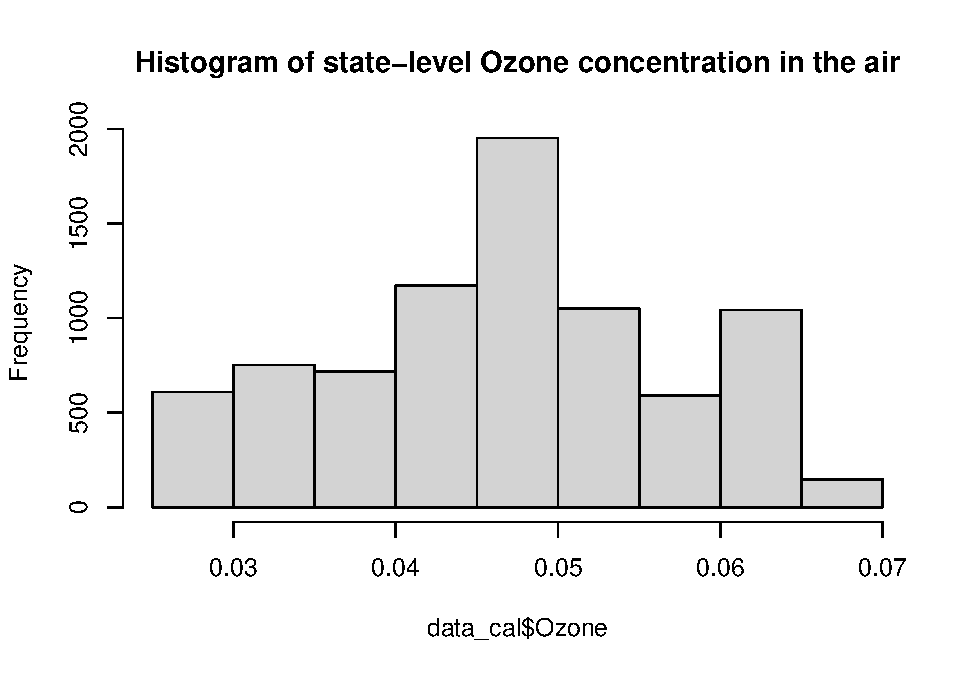
\includegraphics{data_explore_files/figure-latex/unnamed-chunk-6-1.pdf}

\begin{Shaded}
\begin{Highlighting}[]
\CommentTok{\# for the homeless variable, test for colinearity between its three subvariables }
\FunctionTok{pairs}\NormalTok{(soecon}\SpecialCharTok{$}\NormalTok{Total\_poverty }\SpecialCharTok{\textasciitilde{}}\NormalTok{ soecon}\SpecialCharTok{$}\NormalTok{individual\_homeless }\SpecialCharTok{+}\NormalTok{ soecon}\SpecialCharTok{$}\NormalTok{fam\_homeless)}
\end{Highlighting}
\end{Shaded}

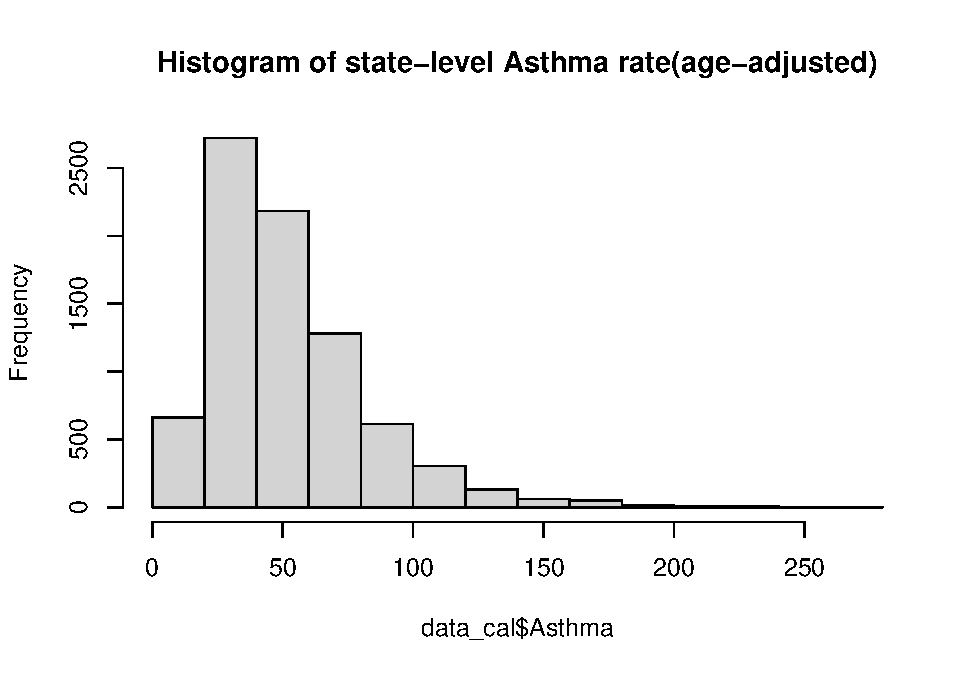
\includegraphics{data_explore_files/figure-latex/unnamed-chunk-7-1.pdf}

\begin{Shaded}
\begin{Highlighting}[]
\NormalTok{fulldat }\OtherTok{\textless{}{-}} \FunctionTok{read\_csv}\NormalTok{(}\StringTok{\textquotesingle{}FullData.csv\textquotesingle{}}\NormalTok{)}
\end{Highlighting}
\end{Shaded}

\begin{verbatim}
## New names:
## Rows: 468 Columns: 42
## -- Column specification
## -------------------------------------------------------- Delimiter: "," chr
## (3): LocationAbbr, LocationDesc, State.Name dbl (39): ...1, YearStart,
## DataValue, LowConfidenceLimit, HighConfidenceLimi...
## i Use `spec()` to retrieve the full column specification for this data. i
## Specify the column types or set `show_col_types = FALSE` to quiet this message.
## * `` -> `...1`
\end{verbatim}

\begin{Shaded}
\begin{Highlighting}[]
\FunctionTok{names}\NormalTok{(fulldat)[}\FunctionTok{names}\NormalTok{(fulldat) }\SpecialCharTok{==} \StringTok{\textquotesingle{}DataValue\textquotesingle{}}\NormalTok{] }\OtherTok{\textless{}{-}} \StringTok{\textquotesingle{}Asthmap\textquotesingle{}}
\FunctionTok{names}\NormalTok{(fulldat)[}\FunctionTok{names}\NormalTok{(fulldat) }\SpecialCharTok{==} \StringTok{\textquotesingle{}TOBDataValue\textquotesingle{}}\NormalTok{] }\OtherTok{\textless{}{-}} \StringTok{\textquotesingle{}TOB\textquotesingle{}}


\CommentTok{\# now we try to determine which variable is more significant in predicting the Asthma prevalence}
\CommentTok{\# forward selection}
\NormalTok{coln }\OtherTok{\textless{}{-}} \FunctionTok{colnames}\NormalTok{(fulldat)}

\NormalTok{coln}
\end{Highlighting}
\end{Shaded}

\begin{verbatim}
##  [1] "...1"                        "YearStart"                  
##  [3] "LocationAbbr"                "LocationDesc"               
##  [5] "Asthmap"                     "LowConfidenceLimit"         
##  [7] "HighConfidenceLimit"         "LocationID"                 
##  [9] "TOB"                         "TOBLowConfidenceLimit"      
## [11] "TOBHighConfidenceLimit"      "AlcHeavyDataValue"          
## [13] "AlcHeavyLowConfidenceLimit"  "AlcHeavyHighConfidenceLimit"
## [15] "AlcBingeDataValue"           "AlcBingeLowConfidenceLimit" 
## [17] "AlcBingeHighConfidenceLimit" "ObeDataValue"               
## [19] "ObeLowConfidenceLimit"       "ObeHighConfidenceLimit"     
## [21] "selfHlthDataValue"           "selfHlthLowConfidenceLimit" 
## [23] "selfHlthHighConfidenceLimit" "HlthCareDataValue"          
## [25] "HlthCareLowConfidenceLimit"  "HlthCareHighConfidenceLimit"
## [27] "X.x"                         "SNAP"                       
## [29] "individual_homeless"         "fam_homeless"               
## [31] "total_homeless"              "unemployment_rate"          
## [33] "Male_poverty"                "Female_poverty"             
## [35] "Total_poverty"               "X.y"                        
## [37] "o3_mean"                     "pm2.5_mean"                 
## [39] "so2_mean"                    "co_mean"                    
## [41] "no2_mean"                    "State.Name"
\end{verbatim}

\begin{Shaded}
\begin{Highlighting}[]
\NormalTok{fulldat }\OtherTok{\textless{}{-}}\NormalTok{ fulldat }\SpecialCharTok{|\textgreater{}} \FunctionTok{drop\_na}\NormalTok{()}

\FunctionTok{require}\NormalTok{(broom)}
\CommentTok{\#forward selection procedure using AIC values }
\NormalTok{lm1 }\OtherTok{\textless{}{-}} \FunctionTok{lm}\NormalTok{(Asthmap }\SpecialCharTok{\textasciitilde{}} \DecValTok{1}\NormalTok{, }\AttributeTok{data=}\NormalTok{fulldat)}
\NormalTok{stepModel }\OtherTok{\textless{}{-}} \FunctionTok{step}\NormalTok{(lm1, }\AttributeTok{direction=}\StringTok{"forward"}\NormalTok{,}
\AttributeTok{scope=}\NormalTok{(}\SpecialCharTok{\textasciitilde{}}\NormalTok{ selfHlthDataValue }\SpecialCharTok{+}\NormalTok{ HlthCareDataValue }\SpecialCharTok{+}\NormalTok{ SNAP}\SpecialCharTok{+}\NormalTok{ individual\_homeless}\SpecialCharTok{+}\NormalTok{fam\_homeless}\SpecialCharTok{+}\NormalTok{total\_homeless}\SpecialCharTok{+}\NormalTok{unemployment\_rate}\SpecialCharTok{+}\NormalTok{Male\_poverty}\SpecialCharTok{+}\NormalTok{Female\_poverty}\SpecialCharTok{+}\NormalTok{Total\_poverty}\SpecialCharTok{+}\NormalTok{o3\_mean}\SpecialCharTok{+}\NormalTok{pm2}\FloatTok{.5}\NormalTok{\_mean}\SpecialCharTok{+}\NormalTok{so2\_mean}\SpecialCharTok{+}\NormalTok{co\_mean}\SpecialCharTok{+}\NormalTok{no2\_mean), }\AttributeTok{data=}\NormalTok{fulldat)}
\end{Highlighting}
\end{Shaded}

\begin{verbatim}
## Start:  AIC=730.7
## Asthmap ~ 1
## 
##                       Df Sum of Sq    RSS    AIC
## + HlthCareDataValue    1    517.58 1843.0 627.51
## + SNAP                 1    234.38 2126.2 688.26
## + Female_poverty       1    168.16 2192.5 701.30
## + Total_poverty        1    156.58 2204.1 703.54
## + individual_homeless  1    141.75 2218.9 706.39
## + Male_poverty         1    132.16 2228.5 708.22
## + total_homeless       1    109.11 2251.5 712.59
## + pm2.5_mean           1     48.19 2312.4 723.94
## + selfHlthDataValue    1     44.27 2316.4 724.66
## + fam_homeless         1     25.34 2335.3 728.12
## + unemployment_rate    1     25.17 2335.5 728.15
## + o3_mean              1     22.64 2338.0 728.61
## + so2_mean             1     18.38 2342.3 729.38
## + co_mean              1     17.73 2342.9 729.50
## + no2_mean             1     12.69 2347.9 730.41
## <none>                             2360.6 730.70
## 
## Step:  AIC=627.51
## Asthmap ~ HlthCareDataValue
## 
##                       Df Sum of Sq    RSS    AIC
## + individual_homeless  1    89.073 1754.0 608.46
## + total_homeless       1    74.204 1768.8 612.05
## + SNAP                 1    73.805 1769.2 612.14
## + unemployment_rate    1    27.231 1815.8 623.19
## + fam_homeless         1    24.571 1818.5 623.81
## + so2_mean             1     9.664 1833.4 627.28
## <none>                             1843.0 627.51
## + no2_mean             1     8.485 1834.6 627.55
## + Female_poverty       1     7.001 1836.0 627.89
## + Total_poverty        1     5.343 1837.7 628.28
## + selfHlthDataValue    1     4.820 1838.2 628.40
## + Male_poverty         1     3.225 1839.8 628.77
## + co_mean              1     1.851 1841.2 629.09
## + pm2.5_mean           1     0.235 1842.8 629.46
## + o3_mean              1     0.067 1843.0 629.50
## 
## Step:  AIC=608.46
## Asthmap ~ HlthCareDataValue + individual_homeless
## 
##                     Df Sum of Sq    RSS    AIC
## + unemployment_rate  1    41.986 1712.0 600.16
## <none>                           1754.0 608.46
## + selfHlthDataValue  1     7.988 1746.0 608.52
## + Female_poverty     1     7.629 1746.3 608.61
## + so2_mean           1     5.785 1748.2 609.06
## + Total_poverty      1     5.276 1748.7 609.18
## + SNAP               1     4.842 1749.1 609.28
## + pm2.5_mean         1     3.445 1750.5 609.62
## + fam_homeless       1     3.108 1750.9 609.71
## + total_homeless     1     3.108 1750.9 609.71
## + Male_poverty       1     2.576 1751.4 609.83
## + no2_mean           1     0.738 1753.2 610.28
## + co_mean            1     0.552 1753.4 610.33
## + o3_mean            1     0.031 1754.0 610.45
## 
## Step:  AIC=600.16
## Asthmap ~ HlthCareDataValue + individual_homeless + unemployment_rate
## 
##                     Df Sum of Sq    RSS    AIC
## + Female_poverty     1   23.6828 1688.3 596.24
## + Total_poverty      1   21.3343 1690.7 596.83
## + Male_poverty       1   16.2212 1695.8 598.12
## + selfHlthDataValue  1   13.7980 1698.2 598.72
## + no2_mean           1    8.0745 1703.9 600.15
## <none>                           1712.0 600.16
## + co_mean            1    6.0010 1706.0 600.67
## + SNAP               1    5.6554 1706.3 600.76
## + so2_mean           1    3.3985 1708.6 601.32
## + fam_homeless       1    1.0034 1711.0 601.91
## + total_homeless     1    1.0034 1711.0 601.91
## + pm2.5_mean         1    0.2104 1711.8 602.11
## + o3_mean            1    0.0011 1712.0 602.16
## 
## Step:  AIC=596.24
## Asthmap ~ HlthCareDataValue + individual_homeless + unemployment_rate + 
##     Female_poverty
## 
##                     Df Sum of Sq    RSS    AIC
## + selfHlthDataValue  1    40.696 1647.6 587.87
## <none>                           1688.3 596.24
## + no2_mean           1     7.661 1680.7 596.31
## + co_mean            1     6.069 1682.2 596.71
## + SNAP               1     3.006 1685.3 597.48
## + so2_mean           1     1.563 1686.8 597.85
## + pm2.5_mean         1     1.072 1687.2 597.97
## + Male_poverty       1     0.909 1687.4 598.01
## + Total_poverty      1     0.834 1687.5 598.03
## + fam_homeless       1     0.705 1687.6 598.06
## + total_homeless     1     0.705 1687.6 598.06
## + o3_mean            1     0.344 1688.0 598.16
## 
## Step:  AIC=587.87
## Asthmap ~ HlthCareDataValue + individual_homeless + unemployment_rate + 
##     Female_poverty + selfHlthDataValue
## 
##                  Df Sum of Sq    RSS    AIC
## + no2_mean        1   23.7578 1623.8 583.70
## + co_mean         1   10.8609 1636.8 587.06
## <none>                        1647.6 587.87
## + SNAP            1    5.9157 1641.7 588.34
## + so2_mean        1    1.9988 1645.6 589.36
## + Male_poverty    1    1.9390 1645.7 589.37
## + Total_poverty   1    1.6508 1646.0 589.45
## + fam_homeless    1    1.5058 1646.1 589.48
## + total_homeless  1    1.5058 1646.1 589.48
## + pm2.5_mean      1    0.6644 1647.0 589.70
## + o3_mean         1    0.3250 1647.3 589.79
## 
## Step:  AIC=583.7
## Asthmap ~ HlthCareDataValue + individual_homeless + unemployment_rate + 
##     Female_poverty + selfHlthDataValue + no2_mean
## 
##                  Df Sum of Sq    RSS    AIC
## <none>                        1623.8 583.70
## + pm2.5_mean      1    6.9724 1616.9 583.87
## + SNAP            1    3.9647 1619.9 584.66
## + Male_poverty    1    2.1987 1621.7 585.12
## + Total_poverty   1    2.1634 1621.7 585.13
## + so2_mean        1    1.4531 1622.4 585.32
## + co_mean         1    1.0612 1622.8 585.42
## + fam_homeless    1    0.9777 1622.9 585.44
## + total_homeless  1    0.9777 1622.9 585.44
## + o3_mean         1    0.1881 1623.7 585.65
\end{verbatim}

\textless\textless\textless\textless\textless\textless\textless{} HEAD

\hypertarget{cdi-data}{%
\paragraph{CDI data}\label{cdi-data}}

\begin{Shaded}
\begin{Highlighting}[]
\FunctionTok{names}\NormalTok{(dat\_full[, }\DecValTok{1}\SpecialCharTok{:}\DecValTok{25}\NormalTok{])}
\end{Highlighting}
\end{Shaded}

\begin{verbatim}
##  [1] "X"                           "YearStart"                  
##  [3] "LocationAbbr"                "LocationDesc"               
##  [5] "DataValue"                   "LowConfidenceLimit"         
##  [7] "HighConfidenceLimit"         "LocationID"                 
##  [9] "TOBDataValue"                "TOBLowConfidenceLimit"      
## [11] "TOBHighConfidenceLimit"      "AlcHeavyDataValue"          
## [13] "AlcHeavyLowConfidenceLimit"  "AlcHeavyHighConfidenceLimit"
## [15] "AlcBingeDataValue"           "AlcBingeLowConfidenceLimit" 
## [17] "AlcBingeHighConfidenceLimit" "ObeDataValue"               
## [19] "ObeLowConfidenceLimit"       "ObeHighConfidenceLimit"     
## [21] "selfHlthDataValue"           "selfHlthLowConfidenceLimit" 
## [23] "selfHlthHighConfidenceLimit" "HlthCareDataValue"          
## [25] "HlthCareLowConfidenceLimit"
\end{verbatim}

\begin{Shaded}
\begin{Highlighting}[]
\NormalTok{dat\_full }\OtherTok{\textless{}{-}} \FunctionTok{read.csv}\NormalTok{(}\StringTok{"FullData.csv"}\NormalTok{)}
\FunctionTok{summary}\NormalTok{(dat\_full[, }\DecValTok{4}\SpecialCharTok{:}\DecValTok{25}\NormalTok{])}
\end{Highlighting}
\end{Shaded}

\begin{verbatim}
##  LocationDesc         DataValue     LowConfidenceLimit HighConfidenceLimit
##  Length:468         Min.   : 6.10   Min.   : 4.200     Min.   : 8.80      
##  Class :character   1st Qu.:10.70   1st Qu.: 8.500     1st Qu.:13.15      
##  Mode  :character   Median :12.10   Median : 9.800     Median :14.90      
##                     Mean   :12.31   Mean   : 9.972     Mean   :15.15      
##                     3rd Qu.:13.80   3rd Qu.:11.350     3rd Qu.:17.00      
##                     Max.   :22.20   Max.   :18.000     Max.   :27.00      
##                     NA's   :1       NA's   :1          NA's   :1          
##    LocationID     TOBDataValue   TOBLowConfidenceLimit TOBHighConfidenceLimit
##  Min.   : 1.00   Min.   : 5.80   Min.   : 4.80         Min.   : 7.00         
##  1st Qu.:16.75   1st Qu.:14.60   1st Qu.:11.95         1st Qu.:17.50         
##  Median :29.50   Median :18.50   Median :15.50         Median :21.80         
##  Mean   :29.79   Mean   :18.61   Mean   :15.75         Mean   :21.88         
##  3rd Qu.:42.50   3rd Qu.:22.40   3rd Qu.:19.30         3rd Qu.:25.95         
##  Max.   :72.00   Max.   :38.30   Max.   :34.50         Max.   :42.20         
##                  NA's   :1       NA's   :1             NA's   :1             
##  AlcHeavyDataValue AlcHeavyLowConfidenceLimit AlcHeavyHighConfidenceLimit
##  Min.   : 2.500    Min.   : 1.500             Min.   : 3.300             
##  1st Qu.: 5.200    1st Qu.: 3.700             1st Qu.: 7.200             
##  Median : 6.300    Median : 4.700             Median : 8.300             
##  Mean   : 6.383    Mean   : 4.722             Mean   : 8.619             
##  3rd Qu.: 7.300    3rd Qu.: 5.500             3rd Qu.: 9.700             
##  Max.   :14.300    Max.   :11.400             Max.   :19.500             
##  NA's   :3         NA's   :3                  NA's   :3                  
##  AlcBingeDataValue AlcBingeLowConfidenceLimit AlcBingeHighConfidenceLimit
##  Min.   : 8.40     Min.   : 5.40              Min.   :10.70              
##  1st Qu.:15.20     1st Qu.:12.55              1st Qu.:18.20              
##  Median :17.90     Median :15.20              Median :21.30              
##  Mean   :18.12     Mean   :15.26              Mean   :21.41              
##  3rd Qu.:20.80     3rd Qu.:17.70              3rd Qu.:24.30              
##  Max.   :32.80     Max.   :27.30              Max.   :39.70              
##  NA's   :1         NA's   :1                  NA's   :1                  
##   ObeDataValue   ObeLowConfidenceLimit ObeHighConfidenceLimit selfHlthDataValue
##  Min.   :39.40   Min.   :34.60         Min.   :43.00          Min.   :78.50    
##  1st Qu.:49.50   1st Qu.:45.20         1st Qu.:53.25          1st Qu.:85.85    
##  Median :53.40   Median :49.20         Median :57.60          Median :87.80    
##  Mean   :53.41   Mean   :49.28         Mean   :57.48          Mean   :87.57    
##  3rd Qu.:57.70   3rd Qu.:53.60         3rd Qu.:61.55          3rd Qu.:89.55    
##  Max.   :69.40   Max.   :64.70         Max.   :74.10          Max.   :95.30    
##  NA's   :1       NA's   :1             NA's   :1              NA's   :1        
##  selfHlthLowConfidenceLimit selfHlthHighConfidenceLimit HlthCareDataValue
##  Min.   :72.70              Min.   :81.5                Min.   :59.60    
##  1st Qu.:82.90              1st Qu.:88.3                1st Qu.:79.30    
##  Median :84.90              Median :90.0                Median :84.50    
##  Mean   :84.73              Mean   :89.9                Mean   :83.61    
##  3rd Qu.:87.20              3rd Qu.:91.6                3rd Qu.:88.90    
##  Max.   :92.90              Max.   :97.0                Max.   :96.50    
##  NA's   :1                  NA's   :1                   NA's   :1        
##  HlthCareLowConfidenceLimit
##  Min.   :56.40             
##  1st Qu.:75.75             
##  Median :81.50             
##  Mean   :80.47             
##  3rd Qu.:85.90             
##  Max.   :94.80             
##  NA's   :1
\end{verbatim}

\begin{Shaded}
\begin{Highlighting}[]
\FunctionTok{hist}\NormalTok{(dat\_full}\SpecialCharTok{$}\NormalTok{DataValue, }\AttributeTok{main=}\StringTok{\textquotesingle{}Histogram of asthma crude prevalence among women aged 18{-}44 years across states\textquotesingle{}}\NormalTok{ )}
\end{Highlighting}
\end{Shaded}

\includegraphics{data_explore_files/figure-latex/unnamed-chunk-11-1.pdf}

\begin{Shaded}
\begin{Highlighting}[]
\FunctionTok{hist}\NormalTok{(dat\_full}\SpecialCharTok{$}\NormalTok{TOBDataValue, }\AttributeTok{main=}\StringTok{\textquotesingle{}Histogram of Percent current cigarette smoking among women aged 18{-}44 years across states\textquotesingle{}}\NormalTok{)}
\end{Highlighting}
\end{Shaded}

\includegraphics{data_explore_files/figure-latex/unnamed-chunk-11-2.pdf}

\begin{Shaded}
\begin{Highlighting}[]
\FunctionTok{hist}\NormalTok{(dat\_full}\SpecialCharTok{$}\NormalTok{selfHlthDataValue, }\AttributeTok{main =} \StringTok{\textquotesingle{}Histogram of Self{-}rated health status among women aged 18{-}44 years across states\textquotesingle{}}\NormalTok{)}
\end{Highlighting}
\end{Shaded}

\includegraphics{data_explore_files/figure-latex/unnamed-chunk-11-3.pdf}

\begin{Shaded}
\begin{Highlighting}[]
\CommentTok{\#air pollutant exploratory}

\FunctionTok{par}\NormalTok{(}\AttributeTok{mfrow =} \FunctionTok{c}\NormalTok{(}\DecValTok{3}\NormalTok{,}\DecValTok{2}\NormalTok{))}
\FunctionTok{plot}\NormalTok{(dat\_full}\SpecialCharTok{$}\NormalTok{DataValue }\SpecialCharTok{\textasciitilde{}}\NormalTok{ dat\_full}\SpecialCharTok{$}\NormalTok{o3\_mean, }\AttributeTok{ylab =} \StringTok{"Asthma Pervalence"}\NormalTok{, }\AttributeTok{xlab =} \StringTok{"Ozone"}\NormalTok{)}
\FunctionTok{plot}\NormalTok{(dat\_full}\SpecialCharTok{$}\NormalTok{DataValue }\SpecialCharTok{\textasciitilde{}}\NormalTok{ dat\_full}\SpecialCharTok{$}\NormalTok{pm2}\FloatTok{.5}\NormalTok{\_mean,}\AttributeTok{ylab =} \StringTok{"Asthma Pervalence"}\NormalTok{, }\AttributeTok{xlab =} \StringTok{"PM2.5"}\NormalTok{)}
\FunctionTok{plot}\NormalTok{(dat\_full}\SpecialCharTok{$}\NormalTok{DataValue }\SpecialCharTok{\textasciitilde{}}\NormalTok{ dat\_full}\SpecialCharTok{$}\NormalTok{so2\_mean,}\AttributeTok{ylab =} \StringTok{"Asthma Pervalence"}\NormalTok{, }\AttributeTok{xlab =} \StringTok{"Sulfur Dioxide"}\NormalTok{)}
\FunctionTok{plot}\NormalTok{(dat\_full}\SpecialCharTok{$}\NormalTok{DataValue }\SpecialCharTok{\textasciitilde{}}\NormalTok{ dat\_full}\SpecialCharTok{$}\NormalTok{co\_mean, }\AttributeTok{ylab =} \StringTok{"Asthma Pervalence"}\NormalTok{, }\AttributeTok{xlab =} \StringTok{"Carbon Monoxide"}\NormalTok{)}
\FunctionTok{plot}\NormalTok{(dat\_full}\SpecialCharTok{$}\NormalTok{DataValue }\SpecialCharTok{\textasciitilde{}}\NormalTok{ dat\_full}\SpecialCharTok{$}\NormalTok{no2\_mean, }\AttributeTok{ylab =} \StringTok{"Asthma Pervalence"}\NormalTok{, }\AttributeTok{xlab =} \StringTok{"Nitrogen Dioxide"}\NormalTok{)}

\FunctionTok{pairs}\NormalTok{(o3\_mean }\SpecialCharTok{\textasciitilde{}}\NormalTok{ pm2}\FloatTok{.5}\NormalTok{\_mean }\SpecialCharTok{+}\NormalTok{ so2\_mean }\SpecialCharTok{+}\NormalTok{ co\_mean }\SpecialCharTok{+}\NormalTok{ no2\_mean, }\AttributeTok{data =}\NormalTok{ dat\_full)}
\end{Highlighting}
\end{Shaded}

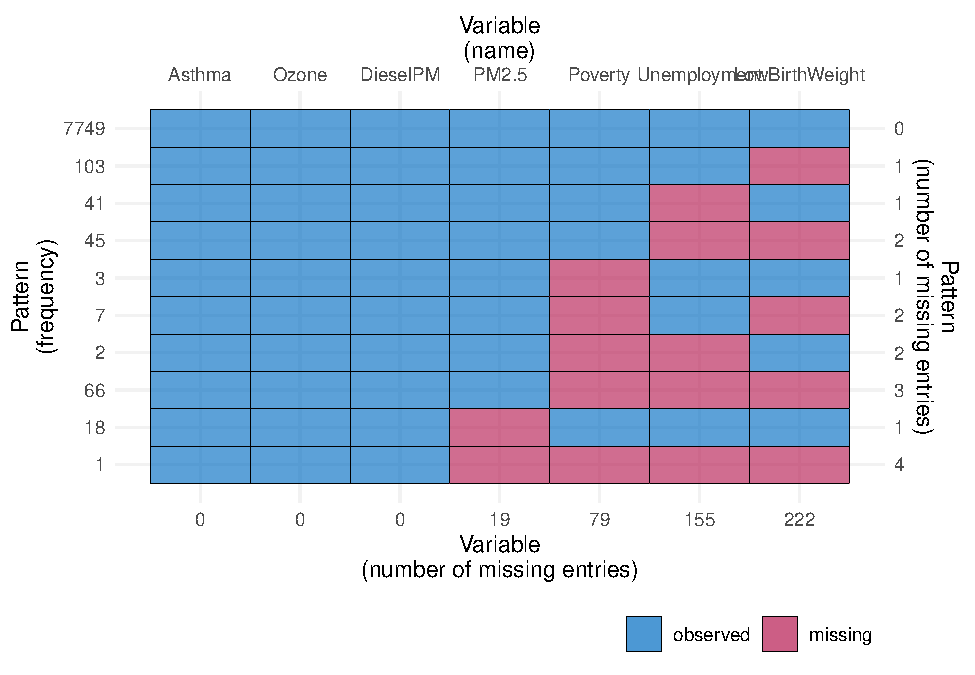
\includegraphics{data_explore_files/figure-latex/unnamed-chunk-12-1.pdf}
\includegraphics{data_explore_files/figure-latex/unnamed-chunk-12-2.pdf}

\end{document}
